\documentclass{article}
\usepackage[UTF8]{ctex}

\usepackage{amsmath, amsthm, amssymb, bm, graphicx, hyperref, mathrsfs}
\title{{\Huge{\textbf{基础物理实验}}}\\测量误差和数据处理}
\author{赵雅鹏\qquad2100011762\\化学与分子工程学院}
\date{\today}
\linespread{1.5}
\newtheorem{theorem}{定理}[section]
\newtheorem{definition}[theorem]{定义}
\newtheorem{lemma}[theorem]{引理}
\newtheorem{corollary}[theorem]{推论}
\newtheorem{example}[theorem]{例}
\newtheorem{proposition}[theorem]{命题}
\usepackage[small]{titlesec}
\usepackage{makecell}


\begin{document}

\maketitle

\pagenumbering{roman}
\setcounter{page}{1}
\newpage
\pagenumbering{Roman}
\setcounter{page}{1}
\setcounter{page}{1}
\pagenumbering{arabic}

\section{数据处理}
%第一题
\subsection{\small 按照表 7-7 列出测量钢杯含钢体积的数据表,并计算出相应的测量结果和不确定度。}
	\[
	\begin{tabular}{|c|c|c|c|}
	\hline
	项目&D/cm&d/cm&H/cm\\
	\hline
	零点读数&$D_{0}=0.000$&$d_0=0.000$&$H_0=0.000$\\
	\hline
	1&2.510&1.684&4.210\\
	\hline
	2&2.512&1.688&4.216\\
	\hline
	3&2.508&1.682&4.214\\
	\hline
	4&2.512&1.686&4.212\\
	\hline
	5&2.512&1.682&4.210\\
	\hline
	6&2.508&1.684&4.210\\
	\hline
	平均值&2.5103&1.6843&4.2120\\
	\hline
	平均值的标准差&0.0008&0.0010&0.0010\\
	\hline
	考虑仪器允差后的标准差&0.0014&0.0015&0.0015\\
	\hline
	修正零点后的平均值&2.5103&1.6843&4.2120\\
	\hline
	\end{tabular}
	\]
游标卡尺允差为\underline{$\pm$0.02mm}\\
测量结果:\\
$\bar{D}\pm\sigma_{\bar{D}}=$\underline{$2.5103\pm0.0008$cm}\\
$\bar{d}\pm\sigma_{\bar{d}}=$\underline{$1.6843\pm0.0015$cm}\\
$\bar{H}\pm\sigma_{\bar{H}}=$\underline{$4.2120\pm0.0015$cm}\\

计算结果:\\
$V=\frac{\pi}{4}(\bar{D}^2-\bar{d}^2)\bar{H}=$\underline{$11.46cm^3$}\\
$\sigma_{V}$(列出公式)=\underline{$ \sqrt{(\dfrac{\partial V}{\partial D}  \sigma_{D})^{2} + (\dfrac{\partial V}{\partial d} *\sigma_{d})^{2} + (\dfrac{\partial V}{\partial H}  \sigma_{H})^{2}  } $}=\underline{$0.03cm^{3}$}\\
$V\pm\sigma_V=\underline{(11.46\pm0.03)cm^3}$


%第二题
\subsection{\small 按照表 7-8 列出测量小钢球体积的数据表,并计算出相应的测量结果和不确定度。(注:\LaTeX 打横向表格空间不够,故此处打纵向表格)}
零点读数$d_0=-0.0003cm$
	\[
	\begin{tabular}{|c|c|}
	\hline
	项目&d/cm\\
	\hline
	1&1.4690\\
	\hline
	2&1.4691\\
	\hline
	3&1.4693\\
	\hline
	4&1.4690\\
	\hline
	5&1.4694\\
	\hline
	6&1.4693\\
	\hline
	平均值&1.46918\\
	\hline
	平均值的标准差&0.00007\\
	\hline
	考虑仪器允差的标准差&0.00024\\
	\hline
	修正零点后的平均值&1.46948\\
	\hline
	\end{tabular}
	\]
螺旋测微器允差为$\pm0.004$mm\\
测量结果:\\
$\bar{d}\pm\sigma_{\bar{d}}=$\underline{1.46948$\pm$0.00024cm}\\

计算结果:\\
$V=\frac{\pi}{6}\bar{d^3}=\underline{1.6615cm^3}$\\
$\sigma_V$(列出公式)=\underline{$ \sqrt{(\dfrac{\partial V}{\partial d}  \sigma_{d})^{2}}$}=\underline{$0.0008cm^3$}\\
$V\pm\sigma_V=\underline{(1.6615\pm0.0008)cm^3}$

\section{习题}

1.
	(1)1位;
	(2)4位;
	(3)2位;
	(4)6位\\

2.    (1)加减法结果不确定度,$\sigma_N=|\dfrac{d\dfrac{1}{x}}{dx}|\times0.1=0.001$,\\
			$\sigma_N=|\dfrac{d\dfrac{1}{x}}{dx}|\times0.1=0.0000001$,方-和-根$\sigma_N=0.001,\\\dfrac{1}{c}=\dfrac{1}{a}-\dfrac{1}{b}=0.100$,c的不确定度$\sigma_N=|\dfrac{d\dfrac{1}{x}}{dx}|\times0.001=0.1$\\ 
			$\therefore c=\dfrac{1}{\frac{1}{a}-\frac{1}{b}}=1.0\times10$\\
\qquad    (2)9.24的不确定度是0.01,\\
结果的不确定度是$\sigma_N>|\dfrac{de^{-x^2}}{dx}|\times0.01=2\times10^{-38}$\\
			$\therefore y=e^{-x^2}=e^{-9.24^2}=8\times10^{-38}$\\
\qquad    (3)56.7的不确定度是0.1,\\
结果的不确定度$\sigma_N>|\dfrac{dlnx}{dx}|\times0.1=0.002$\\
				$\therefore y=lnx=ln56.7=4.038$\\
\qquad    (4)$9^\circ24^\prime$的不确定度是$1^\prime$,\\
结果不确定度$\sigma_N>|\dfrac{dcosx}{dx}|\times1^\prime\times\frac{\pi}{180}=0.00005$\\
$\therefore y=$cos$x=$cos$9^\circ24^\prime$=0.98655\\


3.(b)$\sigma_{\rho}=\sqrt{(\dfrac{\partial \rho}{\partial m_1}\times \sigma_{m_1})^2+(\dfrac{\partial \rho}{\partial m_2}\times\sigma_{m_2})^2}=
\rho_0\times\sqrt{(\dfrac{m_2\sigma_{m_1}}{(m_1-m_2)^2})^2+(\dfrac{m_1\sigma_{m_2}}{(m_1-m_2)^2})^2}=
\dfrac{\rho_0}{(m_1-m_2)^2}\sqrt{m_2^2\sigma_{m_1^2}+m_1^2\sigma_{m_2^2}}$\\
(c) $\sigma_{y}=\sqrt{(\dfrac{\partial y}{\partial a}\times \sigma_a)^2+(\dfrac{\partial y}{\partial b}\times\sigma_b)^2}=\sqrt{((\dfrac{1}{a}-\dfrac{1}{a+b})\sigma_a)^2+((\dfrac{1}{b}-\dfrac{1}{a+b})\sigma_b)^2}
=\dfrac{1}{a+b}\sqrt{\dfrac{b^2\sigma_{a}^2}{a^2}+\dfrac{a^2\sigma_{b}^2}{b^2}}$\\

5.
$\because S=L_1L_2 - \frac{\pi}{4}  d_{1}^{2} - \frac{\pi}{4}  d_{2}^{2}$\\
$\therefore \dfrac{\sigma_{S}}{S} = \sqrt{(\dfrac{\partial \ln(S)}{\partial L_{1}}  \sigma_{L_{1}})^{2} + (\dfrac{\partial \ln(S)}{\partial L_{2}}  \sigma_{L_{2}})^{2} + (\dfrac{\partial \ln(S)}{\partial d_{1}}  \sigma_{d_{1}})^{2} + (\dfrac{\partial \ln(S)}{\partial d_{2}}  \sigma_{d_{2}})^{2} } 
 =\\ \dfrac{1}{L_1L_2 - \frac{\pi}{4}  d_{1}^{2} - \frac{\pi}{4}  d_{2}^{2}}\sqrt{(L_{2}  \sigma_{L_{1}})^{2} + (L_{1}  \sigma_{L_{2}})^{2} + (\dfrac{\pi}{2}  d_{1} \sigma_{d_{1}})^{2} + (\dfrac{\pi}{2} d_{2}  \sigma_{d_{2}})^{2} } $\\
$\because \dfrac{\sigma_{S}}{S} \leq 0.5\%$\\
$\therefore \sigma_{d_2}\leq 0.09$cm\\
$\therefore$ 测量方案是使$d_2$的最后一位的不确定度大于等于$\sigma_{d_2}$,即$0.09$cm

7.
(1)测量结果:$g=\dfrac{2h}{t^2}=980.0\times\dfrac{1+1\times10^{-5}\times10}{(1-1\times10^{-4})^2}=980.3m\cdot s^{-2}$\\
(2)正弦函数二次项以后对准确度的影响远小于二次项,故只考虑二次项\\
第一空:\\
$\because \dfrac{1}{4}sin^2\frac{\theta}{2}\leq0.5\%$\\
$\therefore \theta \leq 16.3^\circ$\\
第一空:\\
$\because \dfrac{1}{4}sin^2\frac{\theta}{2}\leq0.05\%$\\
$\therefore \theta \leq 5.12^\circ$\\

10.(x表示相邻测量点的序号,即用x代替题目中的i以便于表达)\\
$\bar{y}=\dfrac{1}{10} \sum_{i=0}^{10} y_i=66.8571\qquad \bar{x}=\dfrac{1}{10} \sum_{i=0}^{10} x_i=5.5\\ \qquad
\overline{xy}=\dfrac{1}{10} \sum_{i=0}^{10} x_iy_i=439.92 \qquad \bar{x^2}=\dfrac{1}{10} \sum_{i=0}^{10} x_i^2=38.5$\\
$\lambda = \dfrac{\overline{xy}-\bar{x}\bar{y}}{\overline{x^2}-(\bar{x})^2}=\dfrac{439.92-66.8571\times5.5}{38.5-5.5^2}=8.752$(mm)(多保留一位便于更精确计算)\\
$ c= \lambda f \Rightarrow \dfrac{dc}{c}=\dfrac{df}{f}+\dfrac{d\lambda}{\lambda} \Rightarrow
 \dfrac{\sigma_c}{c}=\sqrt{(\dfrac{\sigma_f}{f})^2+(\dfrac{\sigma_\lambda}{\lambda})^2}$\qquad
$\sigma_f=\dfrac{e_f}{\sqrt{3}}$\\
$ r = \dfrac{\sum _{i=1}^{10}(x_{i} - \stackrel{-}{x})\cdot(y_{i} - \stackrel{-}{y})}{\sqrt{\sum _{i=1}^{10}(x_{i} - \stackrel{-}{x})^{2} \cdot \sum _{i=1}^{10}(y_{i} - \stackrel{-}{y})^{2}}} = 0.999969 \\$
随机误差: $\sigma_{\lambda_1} =  \lambda \sqrt{\dfrac{\frac{1}{r^{2}}-1}{n-2}}=0.0244$mm\\
系统误差:$e_1=0.005$mm,\quad$e_2=0.01$mm\\
$\therefore \sigma_\lambda = \sqrt{(\sigma_{\lambda_1})^2+e_1^2+e_2^2}=0.0268$mm \quad$c=\lambda\cdot f = 346.4m\cdot s^{-1}$(多保留一位便于更精确计算)\\
$\therefore \sigma_c = c \cdot\sqrt{(\dfrac{\sigma_f}{f})^2+(\dfrac{\sigma_\lambda}{\lambda})^2} =1.1 $m$\cdot s^{-1} $\\
综上:$\lambda=8.75$mm;\quad c=$364$m/s;\quad$\sigma_c=1.1$m/s\\
11.
(1)\begin{figure}[htbp]
	\centering
	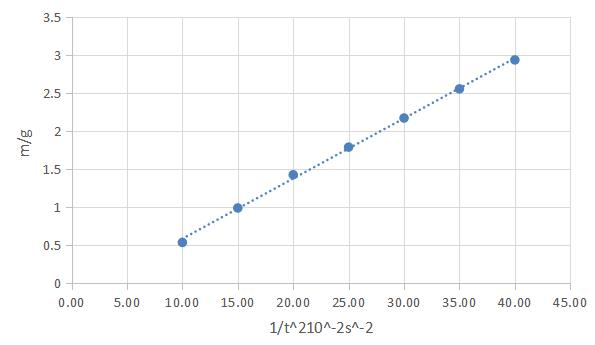
\includegraphics[width=.6\linewidth]{11.jpg}
	\caption{刚体转动实验的线性回归图}
\end{figure}\noindent%
由图2.1知:$m-\dfrac{1}{t^2}$是线性关系\\
(2)令$x=m,y=\dfrac{1}{t^2},$\\
$\bar{x}=\dfrac{1}{7} \sum_{i=0}^7 x_i=25.00\qquad$\quad$\bar{y}=\dfrac{1}{7} \sum_{i=0}^7 y_i=1.7696$\\
$\overline{xy}=\dfrac{1}{7} \sum_{i=0}^{7} x_iy_i=52.142 \qquad \bar{x^2}=\dfrac{1}{7} \sum_{i=0}^{7} x_i^2=725.00$\\$\bar{y^2}=\dfrac{1}{7} \sum_{i=0}^{7} y_i^2=3.7568$\\
$\therefore k_1=\dfrac{\overline{xy}-\bar{x}\bar{y}}{\overline{x^2}-(\bar{x})^2}= \dfrac{52.142-25.00\times1.7696}{725.00-25.00^2}=0.079$\\
$b_1=\bar{y}-k_1\bar{x}=1.7696-0.0079\times25.00=-0.205$\\
$ r_1 = \dfrac{\sum _{i=1}^{7}(x_{i} - \stackrel{-}{x})\cdot(y_{i} - \stackrel{-}{y})}{\sqrt{\sum _{i=1}^{7}(x_{i} - \stackrel{-}{x})^{2} \cdot \sum _{i=1}^{7}(y_{i} - \stackrel{-}{y})^{2}}} = 0.99933 $\\
(3)令$x=\dfrac{1}{t^2},y=m,$\\
$\bar{x}=\dfrac{1}{7} \sum_{i=0}^7 x_i=1.7696\qquad$\quad$\bar{y}=\dfrac{1}{7} \sum_{i=0}^7 y_i=25.00$\\
$\overline{xy}=\dfrac{1}{7} \sum_{i=0}^{7} x_iy_i=52.142 \qquad \bar{x^2}=\dfrac{1}{7} \sum_{i=0}^{7} x_i^2=3.7568$\\$\bar{y^2}=\dfrac{1}{7} \sum_{i=0}^{7} y_i^2=725.00$\\
$\therefore k_2=\dfrac{\overline{xy}-\bar{x}\bar{y}}{\overline{x^2}-(\bar{x})^2}= \dfrac{52.142-25.00\times1.7696}{3.7568-1.7696^2}=12.64$\\
$b_2=\bar{y}-k_2\bar{x}=25.00-12.64\times1.7696=2.63$\\
$ r_2 = \dfrac{\sum _{i=1}^{7}(x_{i} - \stackrel{-}{x})\cdot(y_{i} - \stackrel{-}{y})}{\sqrt{\sum _{i=1}^{7}(x_{i} - \stackrel{-}{x})^{2} \cdot \sum _{i=1}^{7}(y_{i} - \stackrel{-}{y})^{2}}} = 0.99933 $\\

(2)和(3)中的$r_1$和$r_2$相同,因为在相关系数计算的公式中x和y是对称(等价的),因此交换x和y的次序不影响相关系数的计算结果。\\
$k_1,k_2$和相关系数的关系为:\\
\centerline{ $r_1=r_2=\sqrt{k_1k_2}$}

\chapter{分析与讨论}
\section{\small 系统误差和随机误差对于钢杯体积不确定度的贡献.}
$\sigma_{V}$(列出公式)\\={$ \sqrt{(\dfrac{\partial V}{\partial D}  \sigma_{D})^{2} + (\dfrac{\partial V}{\partial d} \sigma_{d})^{2} + (\dfrac{\partial V}{\partial H}  \sigma_{H})^{2}  } $}=$\dfrac{\pi}{4}\sqrt{(2DH  \sigma_D)^2+(2dH\sigma_d)^2+(D^2-d^2)^2\sigma_H^2}$\\
随机误差贡献:$\sigma=\dfrac{\pi}{4}\sqrt{(2\bar{D}\bar{H}  \sigma_{\bar{D}})^2+(2\bar{d}\bar{H}\sigma_{\bar{d}})^2+(\bar{D}^2-\bar{d}^2)^2\sigma_{\bar{H}}^2}=0.020$cm\\
系统误差贡献:$\sigma=\dfrac{\pi}{4}\sqrt{(2\bar{D}\bar{H} \dfrac{e_D}{\sqrt{3}})^2+(2\bar{d}\bar{H}\dfrac{e_d}{\sqrt{3}})^2+(\bar{D}^2-\bar{d}^2)^2(\dfrac{e_H}{\sqrt{3}})^2}=0.015$cm\\
$\because 0.020 > 0.015$\\
$\therefore$ 随机误差对不确定度的贡献比系统误差更大

\subsection{\small 系统误差和随机误差对于小钢球体积不确定度的贡献.}
$\sigma_V=\sqrt{(\dfrac{\partial V}{\partial d}\sigma_d)^2}=\dfrac{\pi}{2}d^2\sigma_d$\\
随机误差贡献:$\sigma_V=\dfrac{\pi}{2}\bar{d}^2\sigma_{\bar{d}}=0.00081$\\
系统误差贡献:$\sigma_V=\dfrac{\pi}{2}\bar{d}^2\dfrac{e}{\sqrt{3}}=0.00078$\\
$\because 0.00081 > 0.00078$\\
$\therefore$ 随机误差对不确定度的贡献比系统误差更大,但二者非常接近,几乎一样\\
\section{收获与感想}
\subsection{有效数字的计算——数学方法和经验方法的异同}
在化学课,如定量分析化学和普通化学中,已经学过关于有效数字的运算规则,但是是一种经验规则,和基础物理实验中的利用数学知识计算的方法算出不准确度的大小再进行有效数字的判断方法不同。但是,用两种方法去进行有效数字的运算,得出的结果基本一致,故可以采用化学课中学习的经验规则而更快地估计有效数字,而数学手段可以作为不确定时的一种检验手段,这样可以加快人工处理数据的速度。
\subsection{关于解决有效数字计算的一些设想}
本次练习误差和数据处理中,牵扯到大量关于有效数字的运算,但是确定有效数字较为繁琐,会使人在分析数据等时精力分散,希望能有计算器的软件可以编程处理有效数字保留位数的问题,让人的注意力可以更多集中在一些更富有创新性生长点的地方,提高效率,减小工作量,也可以提升科研工作者的幸福感和工作与生活质量。

\end{document}










